\pdfoutput=1

\documentclass[12pt]{thesis-umich}[thesis]

\usepackage{url}
\usepackage{graphicx}
\usepackage{subcaption}
\usepackage{amsmath}
\usepackage[inline]{enumitem}
\usepackage{booktabs}
\usepackage{multicol}
\usepackage{color}
\usepackage{booktabs}
\usepackage{multirow}
\usepackage{xspace}
\usepackage{xcolor}
\usepackage{natbib}
\usepackage{amsmath,bm,amsfonts,dsfont,bbm}
\usepackage{hyperref}
\usepackage{mdframed}
\usepackage{csquotes}
\usepackage{epigraph}
\usepackage{geometry}
\usepackage{pdfpages}
\usepackage{graphicx}
\usepackage{fullpage}
\usepackage{amsfonts}
\usepackage{amsmath}
\usepackage{algpseudocode}
\usepackage{algorithm}
\usepackage{subcaption}
\usepackage{amssymb}
\usepackage{appendix}
\usepackage{bbm}
\usepackage{multirow}
\usepackage{pifont}\usepackage{latexsym}

\usepackage{tikz}
\usetikzlibrary{positioning}
\usetikzlibrary{calc}
\usetikzlibrary{arrows}
\usetikzlibrary{decorations.markings}
\usetikzlibrary{shapes.misc}
\usetikzlibrary{matrix,shapes,arrows,fit,tikzmark}
\usetikzlibrary{arrows.meta}
\usetikzlibrary{patterns}
\usetikzlibrary{patterns.meta}
\usetikzlibrary{decorations.pathreplacing,calc,positioning}
\usetikzlibrary{arrows,shapes}
\usetikzlibrary{arrows,chains,positioning,scopes,quotes}
\usetikzlibrary{calc,trees,positioning,arrows,chains,shapes.geometric,decorations.pathreplacing,decorations.pathmorphing,shapes,matrix,shapes.symbols}
\usetikzlibrary{shapes.callouts}
\usepackage[most]{tcolorbox}
\usepackage{array}
\usepackage{colortbl}
\usepackage{dcolumn}
\newcolumntype{d}[1]{D{.}{.}{#1}}  

\usepackage{geometry}
\usepackage[activate={true,nocompatibility}, kerning=true,spacing=true, stretch=10,shrink=30]{microtype}
\microtypecontext{spacing=nonfrench}


\tikzset{
	>=stealth',
	punktchain/.style={
		rectangle, 
		rounded corners, 
		draw=black, text width=5cm, 
		minimum height=2cm, 
		text centered, 
		inner sep=0,outer sep=0,
	},
	line/.style={draw, thick, <-},
	element/.style={
		tape,
		top color=white,
		bottom color=blue!50!black!60!,
		minimum width=8em,
		draw=blue!40!black!90, very thick,
		text width=10em, 
		minimum height=3.5em, 
		text centered, 
		on chain},
	every join/.style={->, thick,shorten >=1pt},
	decoration={brace},
	tuborg/.style={decorate},
	tubnode/.style={midway, right=2pt},
}






\newcommand{\hlent}[2]{\colorbox{gray!20}{#1\textsubscript{#2}}}
\definecolor{dkgreen}{RGB}{0,130,0}
\definecolor{aqua}{rgb}{0.0, 0.4, 1.0}
\setlength{\epigraphwidth}{0.81\textwidth}

\def\vec#1{\ensuremath{\boldsymbol{{#1}}}}
\def\mat#1{\vec{#1}}

\newcommand\BibTeX{B\textsc{ib}\TeX}
\newcommand{\actignore}{\textsc{ignore}\xspace}
\newcommand{\actcoref}{\textsc{coref}\xspace}
\newcommand{\actoverwrite}{\textsc{overwrite}\xspace}
\newcommand{\mysim}{\mathit{sim}}
\newcommand{\mlp}{\mathrm{MLP}}
\newcommand{\cs}{\mathit{cs}}

\newcommand{\unbounded}{U-MEM\xspace}
\newcommand{\learned}{LB-MEM\xspace}
\newcommand{\lru}{RB-MEM\xspace}
\newcommand{\argmax}[1]{\underset{#1}{\operatorname{arg}\,\operatorname{max}}\;}

\newcommand{\bertbase}{BERT\textsubscript{BASE}\xspace}
\newcommand{\bertlarge}{BERT\textsubscript{LARGE}\xspace}

\newcommand*\pct{\scalebox{.8}{\%}}
\newcommand{\pos}[1]{\texttt{#1}}
\newcommand{\reals}{\mathbb{R}}
\newcommand{\legalmove}{LgM\xspace}
\newcommand{\exactmove}{ExM\xspace}
\newcommand{\piecetype}{AP\xspace}

\newenvironment{itemizesquish}{\begin{list}{\setcounter{enumi}{0}\labelitemi}{\setlength{\itemsep}{-0.25em}\setlength{\labelwidth}{0.5em}\setlength{\leftmargin}{\labelwidth}\addtolength{\leftmargin}{\labelsep}}}{\end{list}}

\newenvironment{enumeratesquish}{\begin{list}{\addtocounter{enumi}{1}\labelenumi}{\setlength{\itemsep}{0em}\setlength{\labelwidth}{0.5em}\setlength{\leftmargin}{\labelwidth}\addtolength{\leftmargin}{\labelsep}}}{\end{list}\setcounter{enumi}{0}}

\newcommand{\cmark}{\ding{51}}\newcommand{\xmark}{\ding{55}}
\newcommand{\state}[0]{\texttt{[STATE]}}



\department{Computer Science}

\title{\large{Efficient and Interpretable Neural Models for Entity Tracking}}

\author{Shubham Toshniwal}

\department{Computer Science}

\year=2022

\email{shtoshni@gmail.com}


\frontpagestyle{7} 


\acknowledgments[7]{
The famous proverb "It takes a village to raise a child" is quite apt for my PhD. 
It has been a long winding journey which would've been impossible without some of the smartest, nicest, and hard-working people I've met along the way. 


To begin with, I want to thank Karen Livescu, Kevin Gimpel, and Sam Wiseman. Karen has been my advisor from day one and has been a source of constant support and wisdom throughout these years. I've learned so much from her and am still in awe of her infinite reservoir of calm. 
Karen's meticulousness and research ethics are values that I hope to carry forward in my research career. 
Talking of Kevin, while he officially became my advisor much later, he has guided me from the very start. His love for NLP can rub off on anyone. I'm amazed by his ability to remember even the most minor
details while juggling countless projects. Finally, Sam has been an unofficial third advisor for me. He has been critical to many of this thesis's ideas, which I'm sure he would humbly minimize. I started working with him somewhat late in my Ph.D. which is why I'm envious of his students at
Duke :) Along with Karen, Kevin, and Sam, I want to thank Kenton and Yejin for making time in their busy schedules to be on the thesis committee. 



I want to thank Allyson Ettinger, Mohit Bansal, Liang Lu, and Mrinmaya Sachan with whom I have collaborated during their stints as Research Assistant Professor (RAP) at TTIC. 
Thanks to Tara Sainath and Ron Weiss for being amazing intern hosts at Google in summer of 2017.
Tara and Ron continued to support me beyond my internship and even when I moved away from research in speech. 
Thanks to Daniel Gillick and Alessandro Presta for hosting me at Google in 2018. 

Thanks to Hao Tang, Trang Tran, Kalpesh Krishna, Patrick Xia, Freda Shi, Bowen Shi, and Lingyu Gao for being amazing collaborators. 
Hao is one of the most principled person I've come across and
was lucky to have him as my senior/mentor and for also teaching me tennis. 
With Trang I was involved in one of the most annoying at first but ultimately one of the most satisfying projects during my PhD. 
I've never met Patrick but he is my go to person to talk about coreference. 

Thanks to Hao Tang, Shane Settle, Herman Kamper, Ankita Pasad, Davis Yoshida, Freda Shi, Bowen Shi, David Yunis who made Karen's and SLATTIC group meetings fun and enriching to attend.  
Thanks to my cohort of Ruotian Luo, Rachit Nimavat, Shane Settle, Nick Kolkin, Blake Woodworth, and Falcon Dai with whom I had a lot of fun taking courses and discussing research directions. 
Shane's probably the funniest guy I've met in person and I had an absolute blast attending my initial conferences with him.
Rachit was my first flatmate when I moved to Chicago. 
I'm still searching for someone as carefree and happy as Rachit.
Ruotian was my cubicle neighbor and gosh he could code up things in sleep which I couldn't while awake.
I want to thank Behnam, Shubhendu, Somaya, Haris, and Mrinal for being amazing seniors. Shubhendu, my ex-flatmate, is probably the most interesting person I've met till now. 
I hope his claim of smoking cigars for a long life turns out to be true. 
Thanks to Sudarshan, Andrea, Pushkar, Igor, Ankita, Chip, Kevin, Shashank, Akilesh, Renyu, Omar, Naren, Kshitij for making TTIC a fun place. 
I've bonded with Sudarshan, Pushkar, Ankita, and Shashank over so many topics besides research. 
I want to thank Ankita, Shane, and Sudarshan for proof-reading the thesis. 
I'm grateful to Sudarshan and Igor for bringing in the latest gossip at lightning speeds in the comfort of our cubicles. 
Andrea was my gym/fitness buddy which meant we went to gym a handful of times over the course of our PhDs. 
I'm thankful to Erika and Andrea for inviting me to their elaborate dinners. 

Outside of TTIC, I want to thank my undergraduate friends Baba (Palak), Prof (Prashant), DKM (Dipendra), Gitesh, Gaur (Siddharth), Aritro, Chirag who have been a constant presence even after so many years. 
I want to thank Archita, Palak, Kshiteej, Prashant, Gitesh, Rachit, Udbhav, Sujaya, Jahn, Eeshit for some memorable trips along the way.  

Returning to TTIC, I want to thank Greg and Madhur for teaching two of my favorite courses. TAing for Greg meant seeing more of his humor at close quarters. 
Thanks to Sunanda and Madhur for some fun times outside of work.  
Admininstrators at TTIC have always been top notch and a special shout out to Adam, Chrissy, Amy, and Mary. 
Finally, I want to remember our late ex-president Sadaoki Furui who recently passed away. 
Playing tennis with him was one of the highlights of my PhD. 
We remained in contact till a couple of months back and he was still on top of the latest developments in machine learning.  
I'm still in awe of his youthful energy, humility, and openness. 

I want to thank the city of Chicago, which has such a rich cultural heritage and iconic architecture. 
The view of the Chicago skyline from the lakeshore trail remains one of the most beautiful sights I've ever seen. 
Taking walks along Lake Michigan, Jackson Park, and UChicago campus remain the highlight of my Hyde Park stay. 
Now that I've moved on introducing myself via Chicago has endowed me with an American identity that fills me with pride. 


I want to thank my teachers in DPS Agra and Allen Institute Kota who paved my path to IIT Kanpur. 
In particular, I want to thank Vinod Arora Sir (Principal, DPS Agra), Haraprasad Sahu Sir (Maths, DPS Agra), Jeevan Jyoti Sir (Maths, Allen Kota), and Parijat Sir (Admin, Allen Kota). 
I ended up at both these institutes by sheer luck and they remain seminal in my life trajectory. 

I'm forever indebted to my parents who're still not sure what I do but have unconditionally supported me regardless. 
Mummy and Papa I promise to keep my work a mystery :)
My late grandfather wanted me to become a doctor. He didn't say which one, so I'm counting this one :)
Thanks to my elder brother Arvind and my sister-in-law Neelam for giving us Aadvik and Karthik to pamper.  
While I'm earning the first doctorate in my extended family, the emphasis of education in my upbringing has a big role in that. 
Thanks to my extended family who have always found time for me when I'm back home. 



 }

\committee{ Professor Kevin Gimpel, Co-Chair \\
	Professor Karen Livescu, Co-Chair \\
	Professor Sam Wiseman \\
	Kenton Lee \\
	Professor Yejin Choi \\
} 

\cochair{Co-chair One \& Co-chair Two}

\showlistoftables


\abstract{
	\begin{center}
	{\Large\bf Efficient and Interpretable Neural Models for Entity Tracking} \f(e_i, a, \{s_1, .., s_t\}) = v 0.3em] Transformer}};
	

	\node[on chain, join, minimum height=10cm, inner sep=0cm, outer sep=0cm] (detector){
		
			\renewcommand{\arraystretch}{0.75}
			\setlength{\tabcolsep}{10pt}
			\begin{tabular}{l l l l d{3.2}}
				\texttt{Rafael} & \cellcolor[HTML]{FCA5A5}{} & \cellcolor[HTML]{407F7F}{}  & \cellcolor[HTML]{A5C663}{}  &   1.0\\\\
				\textcolor{ForestGreen}{\texttt{Rafael Nadal}} & \cellcolor[HTML]{45857E}{} & \cellcolor[HTML]{D6B26F}{}  & \cellcolor[HTML]{D16C73}{}  & 5.0 \\\\
				\multicolumn{1}{c}{\vdots} & \multicolumn{3}{c}{\vdots} & \vdots\\\\
				
				\texttt{is} & \cellcolor[HTML]{CB6672}{} & \cellcolor[HTML]{42847D}{}  & \cellcolor[HTML]{86A137}{}   & -10.0 \\\\
				
				\texttt{is the} & \cellcolor[HTML]{9173A9}{} & \cellcolor[HTML]{404040}{}  & \cellcolor[HTML]{D4936B}{}  & -15.0 \\\\
				
				\multicolumn{1}{c}{\vdots} & \multicolumn{3}{c}{\vdots} & \vdots\\\\
				
				\textcolor{ForestGreen}{\texttt{his}} & \cellcolor[HTML]{26547C}{} &
				\cellcolor[HTML]{D6B26F}{}   &
				\cellcolor[HTML]{EF476F}{}  &   3.0 \\\\
				
				\texttt{his toughest} & \cellcolor[HTML]{D4A56B}{} & \cellcolor[HTML]{505F8F}{}  & \cellcolor[HTML]{468C77}{}   &  -1.0 \\\\
				
				\textcolor{ForestGreen}{\texttt{his toughest rival}} & \cellcolor[HTML]{ca0020}{} & \cellcolor[HTML]{f4a582}{}  & \cellcolor[HTML]{404040}{}   &  2.0 \\\\
				
				\multicolumn{1}{c}{\vdots} & \multicolumn{3}{c}{\vdots} & \vdots\\
			\end{tabular}
	};	

		
            \node[above=of detector, yshift=-5mm] (detector_title){
					
					\renewcommand{\arraystretch}{0.75}
					\setlength{\tabcolsep}{10pt}
					\begin{tabular}{l}
						\hspace{0.1in}\Huge{Mention Detector}\\\\
					\end{tabular}
					
				};

			
		
		
	
	
	\node[on chain, join=by {->,"\Large{top- mentions}", text width=3cm, align=center, above, midway}, xshift=20mm, right=of detector, minimum height=3cm, minimum width=3.2cm,  inner sep=0cm, outer sep=0cm] (clustering)
	{
			
			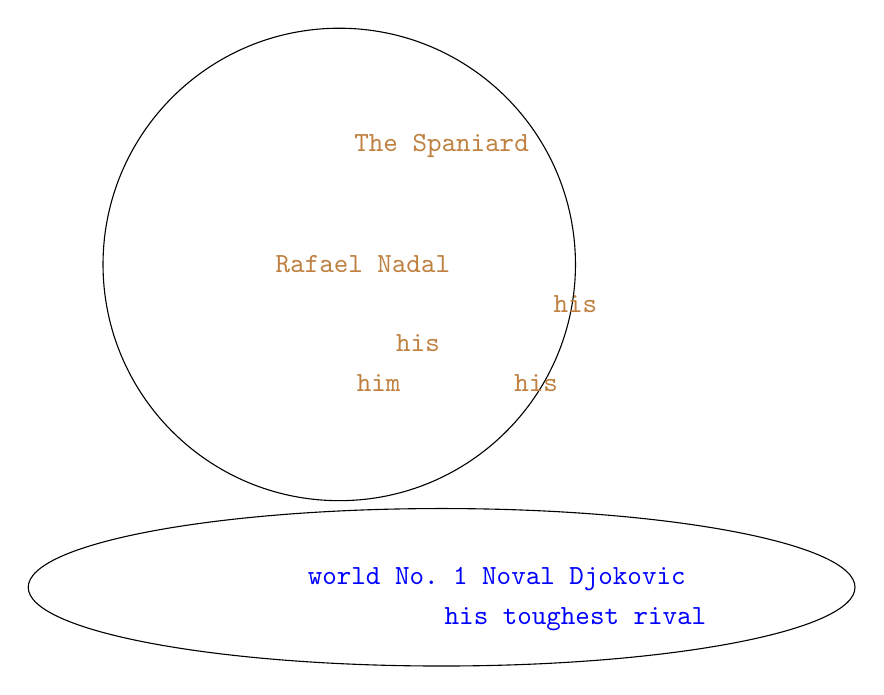
\begin{tikzpicture}[every node/.style={inner sep=0,outer sep=0}]
				\node[circle,
				draw=black,
				text=brown,
				fill=white, minimum size=6cm] (c) at (-0.5,2){};
				\node [font={\ttfamily\color{brown}}] (ment_1) at (-0.2cm, 2cm) {Rafael Nadal}; 
				\node [font={\ttfamily\color{brown}}] (ment_2) at (0.8cm, 3.5cm) {The Spaniard}; 
				\node [font={\ttfamily\color{brown}}] (ment_3) at (0cm, 0.5cm) {him}; 
				\node [font={\ttfamily\color{brown}}] (ment_4) at (0.5cm, 1cm) {his};
				\node [font={\ttfamily\color{brown}}] (ment_5) at (2.5cm, 1.5cm) {his};
				\node [font={\ttfamily\color{brown}}] (ment_6) at (2cm, 0.5cm) {his};
				
				
				\node[ellipse, draw=black, minimum width = 10.5cm, minimum height=2cm] (e) at (0.8,-2.1) {};
				
				\node [font={\ttfamily\color{blue}}] (ment_21) at (2.5cm, -2.5cm) {his toughest rival}; 
				\node [font={\ttfamily\color{blue}}] (ment_22) at (1.5cm, -2cm) {world No.\ 1 Noval Djokovic}; 
			\end{tikzpicture}


	};
				


	
			
			

	
		\node[above=of clustering, right=of detector_title, rectangle,  inner sep=5pt, rounded corners, color=black, very thick] (detector){
			
			\renewcommand{\arraystretch}{0.75}
			\setlength{\tabcolsep}{10pt}
			\begin{tabular}{l}
				\Huge{Mention Clustering}\\\\
			\end{tabular}
			
		};
	
\end{tikzpicture}
}
 \caption{A typical end-to-end coreference pipeline. }
\label{fig:end_to_end_coref}
\end{figure}

Current learning approaches for coreference resolution typically break down the task into two steps, namely \textbf{mention detection} and \textbf{mention clustering} (see Figure~\ref{fig:end_to_end_coref}). 
The mention detection step outputs a pruned set of candidate spans which serve as input to the mention clustering step which finally outputs the entity clusters. 
While earlier state of the art models used a pipeline approach i.e.\ separately learned the two steps~\citep{durrett2013easy,wiseman-etal-2015-learning},  \citet{lee-etal-2017-end} showed the benefits of jointly training the two, which remains a feature in current state of the art models. Since the major algorithmic difference among the approaches lies in the mention clustering step, and is relevant for situating our work, we will briefly overview the four popular clustering approaches (for a more detailed overview, see~\citet{rahman2011narrowing}). 

\begin{enumerate}
	
	\item \emph{Mention-Pair Models}: In this approach, a binary classifier is trained to predict if two candidate mentions are coreferent or not~\citep{mccarthy95decision}. While this approach has been very influential in the past~\citep{soon-etal-2001-machine, ng-cardie-2002-improving, bengtson-roth-2008-understanding}, it has some well-known drawbacks, the most important being the inability to enforce the transitivity property of clustering. 
	For example, even if the classifier predicts mentions  and  to be coreferent, mentions  and  to be coreferent, it can still predict mentions  and  to not be coreferent. The lack of transitivity means that a cluster-decoding algorithm is required by such approaches. Also, the number of binary predictions scales quadratically with the number of mentions which is again undesirable. 
	Finally, since the negative coreference pairs far outnumber the coreferent ones, and the positive pairs which are far apart can be quite hard, under-sampling the negative pairs can be key to performance~\citep{ng-cardie-2002-improving}.  
	
	\item \emph{Mention-Ranking Models}:
	Rather than making pairwise predictions for each mention, mention-ranking models rank \emph{antecedent} mentions for each mention~\citep{durrett2013easy, wiseman-etal-2015-learning, clark-manning-2016-deep, lee-etal-2017-end}. 	This avoids the transitivity issue of mention-pair models as clustering naturally follows from these ranking predictions by chaining together mentions based on their top antecedent picks. 
	Most of the recent state of the art models are based on this paradigm~\citep{joshi-etal-2020-spanbert, xu-choi-2020-revealing}.
	Without any heuristics, the mention-ranking model would keep around all the past mentions in memory, and thus, the runtime would scale quadratically in the number of mentions. Since the number of antecedent mentions can be quite large for long documents, in practice models often use heuristics such as capping the number of candidate antecedents~\citep{lee-etal-2017-end, lee-etal-2018-higher}.

	
	\item \emph{Entity-Mention Models}: The mention-based approaches use only mention-level features which may not be sufficient for accurate classification. The more expressive entity-level features can mitigate this bottleneck. The entity-mention models extend the mention-pair models by  training binary classifiers to predict the linking probability of a mention and a preceding partially formed entity cluster~\citep{luo-etal-2004-mention, yang-etal-2008-entity}. Mentions are merged with the entity-cluster with the highest linking probability.
	
	\item \emph{Entity/Cluster-Ranking Models}:
	While the mention-ranking models lack the entity level features used by entity-mention models, the entity-mention models inherit the drawbacks of pairwise predictions from mention-pair models (except for transitivity). 
	A fix to both of these problems is to incrementally build entity-clusters by  ranking incrementally built entity-clusters for merging a new mention~\citep{rahman2011narrowing, stoyanov-eisner-2012-easy, websterC14, clark-manning-2016-improving}. While entity-ranking models can, in theory, reduce the memory footprint by keeping around only cluster-level representation/features, typical entity-ranking approaches keep around the constituent mentions as well~\citep{rahman2011narrowing, stoyanov-eisner-2012-easy, clark-manning-2015-entity}. Finally, cluster-level features have also been used by mention-ranking approaches which use these  \emph{higher-order} (cluster-level) features along with mention-based features~\citep{wiseman-etal-2016-learning, lee-etal-2017-end, lee-etal-2018-higher, joshi-etal-2019-bert, joshi-etal-2020-spanbert}, though, recent work has questioned the utility of these higher-order features in current models~\citep{xu-choi-2020-revealing}.
	
\end{enumerate}

Some of the recent work in coreference resolution doesn't fit in the above categorization. The current state-of-the-art model by~\citet{wu2019coreference} frames coreference resolution as a question answering (QA) task. The model performs a QA query for each mention and the answer corresponds to all the coreferent spans. Since the number of mentions can be linear in document length, this model scales poorly with the length of document. 
\citet{paolini2021structured} model coreference resolution, and other structured prediction tasks, as a translation task. 
\citet{kirstain-etal-2021-coreference} and \citet{dobrovolskii-2021-word} propose methods which avoid an explicit mention detection step i.e.\ filtering of top candidate spans. 


In this thesis, we propose memory models (Section~\ref{sec:memory_model}) which adopt the entity-ranking paradigm  (Chapters 3 and 4). The external memory in these models tracks the entities where entities are represented via a fixed-dimensional vector representation.   






\subsection{Evaluation Metrics}
Evaluating the performance of an individual coreference link, which is just a binary classification problem, can be done by standard measures such as F-score. However, the full coreference resolution task, which we view as a clustering task, has no such clear evaluation. 
For example, it's not clear if adding/deleting a mention to/from a larger cluster should incur more penalty than the same action performed on a smaller cluster. Similarly,  how should penalty for a mention missed in a cluster compare with that of a spurious mention added to a cluster. 
In fact, the evaluation is even more challenging than a typical clustering task because the system output won't necessarily be perfect on mention detection, and thus, the system output and ground truth would differ even on the clustered elements.


Below we briefly discuss the three metrics, namely MUC~\citep{vilain-etal-1995-model}, B\textsuperscript{3}~\citep{Bagga98algorithmsfor}, and ~\citep{luo-2005-coreference},  used in the coreference resolution literature. All three metrics define precision, recall, and F-score based on a quantity of interest. 
While these three metrics have known shortcomings~\citep{Bagga98algorithmsfor, luo-2005-coreference,  moosavi-strube-2016-coreference}, and the agreement between the them is low~\citep{holen-2013-critical}, we'll follow the proposal by \citet{denis09global}  of averaging the F-score of the three metrics, which is the popular metric of choice and is referred to as CoNLL F-score in the literature. We describe the three metrics next.

In the following discussion, assume  to represent the gold truth entity set and  to represent the predicted entity set. Each element in  and  represents an entity which is represented as a mention set. Finally, let  denote the size of set . 

\paragraph{MUC} is a link-based metric. It uses the number of links preserved for entity sets. MUC recall is defined as:

where  denotes the entity sets in  across which mentions of  are present. Thus, the recall is lower, if entity  is split across multiple predicted clusters in . 
MUC precision is computed by reversing the roles of  and . 
The MUC metric is known to prefer outputs with over-merged entities as they lead to higher recall ~\cite{luo-2005-coreference}.  

\paragraph{B\textsuperscript{3}} is a mention-based metric. For an entity , it uses the fraction of mentions in  present in predicted entities in . Formally, B\textsuperscript{3} recall is defined as: 



As in MUC, B\textsuperscript{3} precision is computed by reversing the roles of  and . Two known shortcomings of B\textsuperscript{3} are that:  (a)  the  B\textsuperscript{3} recall is 100\% if the system output merges all the gold mentions, and (b) the  B\textsuperscript{3} precision is 100\% if the system predicts every gold mention to be a singleton. 

\paragraph{} metric assumes that one gold entity should map to one system entity and vice-versa. It uses the similarity metric  to calculate a one-to-one alignment between  and . The similarity for a gold entity  and system entity  is given by:

Assuming  to be the set of gold entities included in the optimal entity mapping OPT, the  recall is given by:

where OPT represents the optimal mapping of entity  in . For calculating precision, the denominator is changed to  . 













 \section{Entity Tracking}
Entity tracking refers to the broad umbrella of tasks concerning maintaining the entities and their attributes. Typically what constitutes an entity state is dataset-specific which means that the task is arguably less standardized than a typical linguistic task. 


The usual approach to an entity tracking task is by training a supervised model on datasets annotated with entity states. The supervision can be in the form of question answers as in the bAbI tasks~\cite{weston2015aicomplete} and ProPara task~\cite{dalvi-etal-2018-tracking}, or in the form of classification task as in the Recipes task~\cite{kiddon-etal-2016-globally, bosselut-18}. 
Recent work by \citet{tandon-etal-2020-dataset} explores a generative task where given a sentence in the context of a procedural text, the task is to generate the state changes for all the entities involved. 
\citet{henaff2016tracking} proposed EntNet, a model which is equipped with an external memory to track entities mentioned in the discourse. 
\citet{bosselut-18} proposed Neural Process Networks (NPN), a memory model, where the model learns to simulate the action dynamics i.e.\ how the entity states change when an action is applied. The setup assumes that the entities mentioned in a discourse are given and the set of actions is known a priori while training. These simplifying assumptions severely limit the applicability of NPN beyond the Recipes task used in the work. \citet{gupta-durrett-2019-tracking} propose a structured architecture for tracking the observable discrete attributes, such as location, and the unobserved implicit entity state. Moving away from explicit entity-centric memory representations, \citet{gupta-durrett-2019-effective} explore the use of pretrained transformers for entity tracking in  the ProPara and Recipes datasets. While transformers outperform prior work, their error analysis shows that transformer-based models mostly rely on surface clues and don't form accurate intermediate entity representations.   

Entity tracking has also been explored for the cloze task LAMBADA~\cite{paperno-etal-2016-lambada}, where  the task is to predict the last word of a passage (\emph{cloze tasks} refers to tasks where the goal is to fill in the missing language item). The task instances were filtered such that succeeding on the task requires understanding the whole passage  instead of just the local context. 
\citet{chu-etal-2017-broad} conducted an manual analysis of the LAMBADA validation set which showed that roughly 20\% of the instances require coreference resolution. This analysis led to work, such as \citet{dhingra-etal-2018-neural} and \citet{hoang-etal-2018-entity}, where they utilize entity tracking related information in their models.  \citet{cheng2020entity} introduce a loss to promote attending to  coreferential mentions while processing mentions of the same coreference chain. 

There has been a rich line of work exploring entity tracking in tandem with language models. \citet{ji-etal-2017-dynamic} propose the EntityNLM language model which augments the LSTM network with an entity-centric external memory. \citet{clark-etal-2018-neural} extend the EntityNLM model for story generation. 
\citet{liu2019referential} propose the Referential Reader which is trained on both a sparsely annotated coreference resolution dataset and the language modeling task. Ablation studies for the Referential Reader show that the language modeling task aids entity tracking. 

There has been an ongoing debate on how much \emph{meaning} language models can learn given that they are just trained on text \emph{symbols}~\cite{bender-koller-2020-climbing, Bender2021OnTD}. The literature is divided with regards to entity tracking capabilities of pretrained language models.
\citet{li-etal-2021-implicit} demonstrate, via the use of probing classifiers (Section~\ref{sec:probing_classifier}), that pretrained transformer LMs implicitly learn to track entities. 
On the contrary, \citet{schuster-linzen-2022-sentence} show that even models at the scale of GPT-3 struggle with basic entity tracking capabilities, though scaling up does seem to aid these capabilities.
\citet{sorodoc-etal-2020-probing} show via probing analysis that transformer LMs lack a global notion of entities. \citet{tenney2019probing} use the ``edge probing'' framework (see Section~\ref{sec:probing_intro}) to diagnose linguistic capabilities of different pretrained LMs and find that models are better at capturing syntax than entity-centric information like coreference. 


 
\section{Probing}
\label{sec:probing_intro}
The black box nature of neural models has given rise to a rich area of work on interpretability and analysis of neural NLP models. 
Interpretability is an important aspect of this thesis, especially for our work on integrating entity tracking into language models.
In this section, we discuss probing methods which refers to a broad umbrella of analysis techniques. 
For this discussion, we first discuss two prominent probing methods in the literature, namely \emph{diagnostic probing} and \emph{behavioral probing}. Finally, we discuss the emerging area of \emph{probing via prompting} which has the most relevance to this thesis.  

\subsection{Diagnostic Probing}
\label{sec:probing_classifier}
In diagnostic probing, a supervised probing classifier is trained on the internal representations of the model of interest to predict an external property. 
A high-performing probing classifier is assumed to imply that the external property is represented in the model and vice-versa. 
Typical design decisions in this probing mechanism involve the choice of: (a) probing classifier (linear, multilayer perceptron, etc.), (b) internal representation (which layer to use, how to reduce the representation to a fixed dimension), and (c) the amount of supervision used. 

Diagnostic probing has been one of the most popular probing methodologies in the literature, with an extensive use for probing for linguistic properties. 
\citet{ettinger-etal-2016-probing} and  ~\citet{adi17probing} use probing classifiers for analysis of sentence embeddings. \citet{belinkov-etal-2017-neural} analyze the representation of machine translation models for morphological tasks. \citet{liu-etal-2019-linguistic, tenney-etal-2019-bert} and ~\citet{tenney2019probing} use probing classifiers to diagnose the transformer layers of various pretrained LMs for various linguistic tasks.  
  




Despite its popularity, the diagnostic probing methodology has some critical shortcomings. 
One of the most important shortcoming is what to attribute the performance of a probing classifier to? 
A high-performing probing classifier could be because the model representation indeed captures the property of interest, but it could also be because the probing classifier has learned the probing task.  
\citet{hewitt-liang-2019-designing} argue for probes which are more ``selective'' i.e. ones which are high-performing for the task of interest but have a low performance for a control task constructed by randomizing  input-output pairs from the task of interest.  
In contrast, \citet{pimentel-etal-2020-information} argue on information-theoretic principles that the best performing probing model, even if it's more complex, should be used.  
Another shortcoming of probing classifiers is that while they can reveal what information is present in the model's representation, they don't say anything about whether the model is using this information in actual downstream tasks. 
Ongoing work is trying to address these shortcomings. 
For a detailed overview of probing classifiers, we refer the reader to the recently published survey by \citet{belinkov2022probing}. 


\subsection{Behavioral Probing}
 \nocite{goldberg2019assessing}  
In behavioral probing, analysis is carried out typically by observing the model's predictions i.e.\ behavior. 
To this end, evaluation sets are created to tease apart the model's performance. 
The evaluation datasets can be hand-crafted~\cite{ettinger-2020-bert}, automatically created~\cite{gulordava-etal-2018-colorless}, or obtained by filtering from a naturally occurring corpus~\cite{linzen-etal-2016-assessing}. 
In \citet{linzen-etal-2016-assessing}, the authors study the subject-verb agreement for a LSTM language model for sentences filtered from Wikipedia. 
\citet{marvin-linzen-2018-targeted} construct minimally different sentence pairs, consisting of an ungrammatical and grammatical sentence, to evaluate the grammatical preference of language models. \citet{ettinger-2020-bert} propose and perform a suite of psycholinguistic evaluations for diagnosing BERT, with one of the surprising findings being BERT's insensitivity to negation~\cite{Fischler1983BrainPR}.
 
While behavioral probing avoids introducing the confound of a probing classifier, as in diagnostic probing, it is limited by what can be probed by observing the model's behavior. Moreover, in the case of hand-curated datasets, constructing the dataset can be costly, which often limits the size of these tests to merely hundreds of examples~\cite{Fischler1983BrainPR, chow2015bag}. Finally, because the output space of model predictions may not be constrained, models can make reasonable predictions that are not covered by the hand-curated datasets and thus will be wrongly penalized by evaluations~\cite{lialin-etal-2022-life}.

\subsection{Probing via Prompting}
Prompting has emerged as a new modeling methodology which employs pretrained generative LMs~\cite{brown2020language, Liu2021PretrainPA}. 
Recent work has started exploring prompting for probing as well~\cite{toshniwal-etal-2022-chess, li-etal-2022-probing-via}. 
In this methodology, the probing task of interest is verbalized i.e.\ converted to text tokens, and trained along with the task of language modeling. 
The formulation assumes: (a) the probing task can be verbalized, and (b) the language model can be finetuned (which can be computationally infeasible for some of the big language models like GPT-3).  
Compared to diagnostic probing, a benefit of this formulation is that it avoids the hassle of selecting a probing classifier. And since the LM is finetuned for the probing task, the LM outputs tend to be more constrained in comparison to behavioral probing. 
We use the probing via prompting framework to diagnose the entity tracking capability of transformer LMs in Chapters 5 and 6 of this thesis. 




 
\section{Memory Models}
\label{sec:memory_model}
Memory models refer to end-to-end differentiable neural networks coupled with an external memory~\cite{graves2014neural,graves2016hybrid}. 
The external memory can be thought of like a Turing tape~\cite{turing1950mind}, or when viewed through the lens of cognitive psychology, as \emph{working memory}~\cite{baddeley1986} (see \citet{Nematzadeh2020ONMI} for a discussion on the different memory types). 
The decoupling of the model parameters from the external memory means that a memory model can have an arbitrarily large memory without increasing the model parameters.\footnote{There are variants of memory models where the external memory is parameterized.}  
This differentiates memory models from recurrent neural networks such as  Long Short-Term Memory (LSTM)~\cite{hochreiter1997long} where the parameters grow quadratically with the memory size (memory cell size). 

\begin{figure}[t]
    \centering
    \includegraphics[scale=0.35]{figures/background/ntm_clean.pdf}
    \caption{Schematic figure of the Neural Turing Machine. Source \citet{graves2014neural}.}
    \label{fig:ntm}
\end{figure}

Neural Turing Machine (NTM), shown in Figure~\ref{fig:ntm}, represents one of the first memory models proposed in the literature~\cite{graves2014neural}. 
The NTM model proposed two key abstractions, namely controller and memory. 
The controller receives an external input, such as the next word or the next sentence. Conditioned on this external input, the controller reads the memory state,  then combines the external input and the read memory to produce: (a) a write update for the memory and (b) an external output. 
While the exact implementation details of the model have been modified in follow-up work, the abstractions presented in the NTM work have largely persisted. We discuss the memory model components and design choices next.  

\subsection{Memory Model Details}
In this section, we discuss the key memory model components and associated design choices. 

\paragraph{Memory} There are various design choices associated with memory, such as the memory structure, the memory size, the memory initialization, etc. For a typical memory model, the memory can represented via a matrix  where  represents the number of memory cells and  represents the size of each memory cell. 
The memory size  can be unbounded~\cite{weston2014memory, graves2014neural} or bounded~\cite{sukhbaatar-15, henaff2016tracking}. 
Each memory cell can simply be a -dimensional vector~\cite{weston2014memory, sukhbaatar-15} or have a key-value structure where the -dimensional vector is split into two fixed-dimensional parts, namely key and value~\cite{miller-etal-2016-key, henaff2016tracking, liu2019referential}. 
At inference time, the memory cells could be initialized to a fixed/random vector~\cite{graves2014neural, sukhbaatar-15, graves2016hybrid} or the initialization could be learned~\cite{henaff2016tracking, liu2019referential}.

\paragraph{Memory Reading and Writing}
Given the input  at time step , the controller uses read head(s) to attend to the memory . Typically the memory models use content-based addressing where the read head(s) use a  similarity measure between the memory units and the input to retrieve  memories ``similar'' to an input. Models such as Differentiable Neural Controller (DNC)~\cite{graves2016hybrid} also support spatial and temporal memory access. For the content-based reading mechanism, a typical implementation does the following:

where  represents the th memory cell at timestep  and the function  represents a similarity function. This \emph{soft} reading mechanism has been commonly used in prior work, including NTM and DNC. A simple tweak to the \emph{soft} reading mechanism is to use the top- scoring memory units~\cite{weston2014memory}.  
To support scalable memory reads, prior work has also proposed sparse read mechanisms based on approximate nearest neighbor search~\cite{weston2014memory, rae2016scaling}. 


Memory write operations are required to store information which can be retrieved in later read operations. The memory update function has the form: 

The write operation, similar to the read operation, could have a \emph{soft} update where all the memories are overwritten~\cite{graves2014neural, graves2016hybrid, liu2019referential, henaff2016tracking} or a \emph{hard} update where a select few memory units are updated~\cite{rae2016scaling}. The criteria for selecting which memory unit to write to could be based on content-based similarity or based on the least recently used memory units~\cite{rae2016scaling}. If there are no memory size constraints, another simple write operation is to keep appending to the memory for every input~\cite{weston2014memory}.    









\subsection{Application of Memory Models in NLP}


Some of the earliest applications of memory networks in NLP were for question answering, where the external memory simply stored all of the word/sentence embeddings for a document~\cite{weston2014memory, sukhbaatar-15, kumar2016ask, miller-etal-2016-key, henaff2016tracking}. 
Since then, memory models have been applied to several other NLP tasks in addition to question answering, including aspect-based sentiment analysis~\citep{liu-etal-2018-recurrent}, machine translation~\citep{maruf-haffari-2018-document}, narrative modeling~\citep{liu-etal-2018-narrative}, coreference resolution~\cite{liu2019referential}, and dialog state tracking~\citep{perez-liu-2017-dialog}. 
Story generation models have augmented language models with external memory which is meant to track the evolving entity state~\cite{clark-etal-2018-neural, rashkin-etal-2020-plotmachines}. 

In this thesis we explore memory models for the coreference resolution task in Chapters 3 and 4. 
The memory cells in these models are used for tracking entity cluster representations. 
In Chapter 3 we propose a \emph{soft} read and \emph{soft} write memory model. 
We show that learning memory initialization in our setup leads to worse performance and more model parameters.   
In Chapter 4 we propose a \emph{hard} read and \emph{hard} write memory model. In Chapter 3 the proposed memory model only has bounded memory while in Chapter 4 we explore both unbounded and bounded memory models.  








 \section{Pretrained Language Models}
In this section, we briefly overview pretrained language models. Pretrained LMs have lately become ubiquitous in NLP pipelines and are extensively used in this thesis as well. 
These LMs are trained on massive corpora, such as C4~\cite{raffel-etal-2020-exploring}, with self-supervised losses, such as masked LM loss~\cite{devlin-etal-2019-bert, joshi-etal-2020-spanbert}, autoregressive LM loss~\cite{radford2019language}, next sentence prediction loss~\cite{devlin2019bert}, sentence permutation loss~\cite{lewis-etal-2020-bart}. 
We limit our discussion to the model architecture of different pretrained LMs since that has the most relevance for this thesis. For a detailed discussion on pretrained LMs, we refer the reader to \citet{qiu2020ptmsurvey}. 


\paragraph{Model Architecture} 

The pretrained LM paradigm has largely coincided with the emergence of the Transformer~\cite{vaswani2017attention} as the \emph{prima} network in NLP. Hence, since some of the earlier pretrained LMs, such as ELMo~\cite{peters-etal-2018-deep} and CoVe~\cite{mccann2017cove}, which used LSTM~\cite{hochreiter1997long}, almost all the popular pretrained LMs are based on the transformer network. The three main transformer-based LM architectures proposed by prior work are:
\begin{itemize}
    \item \emph{Encoder-only}: 
    This class of LMs includes the BERT model~\cite{devlin-etal-2019-bert} and its follow-ups~\citep[\emph{inter alia}]{joshi-etal-2019-bert, liu-etal-2019-roberta}. The LMs in this category are used as feature extractors for NLP tasks like question answering~\cite{karpukhin-etal-2020-dense}, text classification~\cite{sun2019fine}, coreference resolution~\cite{joshi-etal-2019-bert}. 
    \item \emph{Decoder-only}: The most popular class of LMs from this category is the GPT family of models~\cite{radford2018improving, radford2019language, brown2020language}. The decoder-only LMs have previously been used for text generation tasks, such as story generation~\cite{rashkin-etal-2020-plotmachines}, multiple choice question answering~\cite{radford2018improving}. Recently an interesting avenue of prompt-based learning has emerged with GPT-3 scale models~\cite{lester-etal-2021-power, li-liang-2021-prefix}.
    \item \emph{Encoder-Decoder}: The encoder-decoder LMs generalize the encoder-only and decoder-only architectures. Some of the popular models in this family include BART~\cite{lewis-etal-2020-bart} and T5~\cite{raffel-etal-2020-exploring}. These models are commonly used for conditional generation tasks, such as summarization, machine translation, etc.  
\end{itemize}





In this thesis we use: (a) the BERT model~\cite{devlin-etal-2019-bert} in Chapter 3, (b) the Longformer model~\cite{beltagy2020longformer} in Chapter 4, (c) the GPT-2 model~\cite{radford2019language} in Chapter 5 and 6 (in Chapter 5 we only use the architecture of GPT-2), and (d) the BART model~\cite{lewis-etal-2020-bart} in Chapter 6. In most of the cases, we have finetuned the pretrained models. We have released the trained LMs from Chapter 4 and 5 on Hugging Face model hub.\footnote{\url{https://huggingface.co/shtoshni}}          
 \chapter{PeTra: A Sparsely Supervised Memory Model for People Tracking}
\epigraph{
	\footnotesize{
		Consider a device designed to read a text in some natural language, interpret it, and store the content in some manner, say, for the purpose of being able to answer questions about it. To accomplish this task, the machine will have to fulfill at least the following basic requirement. It has to be able to build a file that consists of records of all the individuals, that is, events, objects, etc., mentioned in the text and for each individual record whatever is said about it.
}}{\textit{Lauri Karttunen, 1976}}

\begin{figure*}[ht]
    \centering
     \includegraphics[width=\textwidth]{figures/petra/sample_run.pdf}
     \captionof{figure}{Illustration of memory cell updates in an example sentence where IG = ignore, OW = overwrite, CR = coref. Different patterns indicate the different entities, and an empty pattern indicates that the cell has not been used. The updated memory cells at each time step are highlighted.
     }
     \label{fig:ideal_run}
\end{figure*}

\section{Introduction}
In this chapter, we introduce PeTra, a bounded memory model, which is trained with the sparse supervision of the GAP (Gendered Ambiguous Pronouns) pronoun resolution task~\citep{webster2018gap}. 
Since we train the model on the pronoun resolution task, the task of entity tracking is reduced to just people tracking which is where Pe(ople)Tra(cking) derives its name from. 
PeTra is inspired by the Referential Reader model from \citet{liu2019referential} but is substantially simpler. In terms of evaluation, apart from the end-task evaluation of pronoun resolution, we also investigate the interpretability and generalization capabilities of memory models by testing if they are indeed tracking people in their memories. For this end, we: (a) propose a new diagnostic evaluation based on counting the number of unique entities in text, and (b) conduct a small scale human evaluation to compare evidence of people tracking in the memory logs of PeTra relative to the Referential Reader. 

Despite using  a simpler architecture, PeTra outperforms the Referential Reader on the end task of pronoun resolution.  
Importantly, while Referential Reader performance degrades with larger memory, PeTra improves with increase in memory capacity (before saturation).
Moreover,  we find PeTra to be highly effective in the interpretability evaluations, especially the human evaluation where annotators overwhelmingly favor PeTra in comparison to the Referential Reader.\footnote{The material in this section is adapted from \citet{toshniwal2020petra}.}
\footnote{Code available at \url{https://github.com/shtoshni/petra}.}



\section{Model}


Figure~\ref{fig:model_sch} depicts PeTra, which
consists of three components: an {\it input encoder} that given the tokens generates the token embeddings, a {\it memory module} that tracks information about the entities present in the text, and a {\it controller network} that acts as an interface between the encoder and the memory.
\begin{figure}[th]
	\centering
	\includegraphics[width=0.4\textwidth]{figures/petra/model_fig.pdf}
	\captionof{figure}{Proposed model.}
	\label{fig:model_sch}
\end{figure}


\subsection{Input Encoder}
\label{sec:input_encoder}
Given a document consisting of a sequence of tokens , we first pass the document through a fixed pretrained BERT model~\cite{devlin2019bert} to extract contextual token embeddings.
Next, the BERT-based token embeddings are fed into a single-layer unidirectional Gated Recurrent Unit (GRU) ~\cite{cho2014learning} running left-to-right to get task-specific token embeddings .

\subsection{Memory}
The memory  consists of  memory cells. The  memory cell state at time step  consists of a tuple 
where the vector  represents the content of the memory cell, and the scalar  represents
its recency of usage. A high value of  is intended to mean that the cell is tracking an entity that has been recently mentioned. 

\paragraph{Initialization}
Memory cells are initialized to the null tuple, i.e.\ (\vec{0}, 0); thus, our memory is parameter-free. This is in contrast with previous entity tracking models such as EntNet~\cite{henaff2016tracking} and the Referential Reader~\cite{liu2019referential} where memory initialization is learned and the cells are represented with separate {\it key} and {\it value} vectors.
We will later discuss variants of our memory with some of these changes.




\subsection{Controller}
At each time step  the controller network determines whether token  is part of an entity span and, if so, whether the token is coreferent with any of the entities already being tracked by the memory. Depending on these two
variables, there are three possible actions: \begin{enumerate}[label=(\roman*)]
	\itemsep0em
	\item \actignore: The token is not part of any entity span, in which case we simply ignore it.
	\item \actoverwrite: The token is part of an entity span \emph{but} is not already being tracked in the memory.
	\item \actcoref: The token is part of an entity span and the entity is being tracked in the memory.
\end{enumerate}
Therefore, the two ways of updating the memory are \actoverwrite and \actcoref.
There is a strict ordering constraint to the two operations: \actoverwrite precedes \actcoref, because it is not possible to corefer with a memory cell that is not yet tracking anything. That is, the \actcoref operation cannot be applied to a previously unwritten memory cell, i.e.~one with . Figure~\ref{fig:ideal_run} illustrates an idealized version of this process.

Next we describe in detail the computation of the probabilities of the two operations for each memory cell at each time step .

First, the {\bf entity mention probability} , which reflects the probability that the current token  is part of an entity mention, is computed by:

where  is a multi-layer perceptron and  is the logistic function.

\paragraph{Overwrite and Coref}
If the current token  is part of an entity mention, we need to determine whether it corresponds to an entity being currently tracked by the memory or not.
For this we compute the similarity between the token embedding  and the contents of the memory cells currently tracking entities.
For the  memory cell with memory vector  the similarity with  is given by:
where  is a second MLP and  is the Hadamard (elementwise) product.
The usage scalar  in the above expression provides a notion of distance between the last mention of the entity in cell  and the potential current mention.
The higher the value of , the more likely
there was a recent mention of the entity being tracked by the cell.
Thus  provides an alternative to distance-based features commonly used in pairwise scores for spans
\citep{lee-etal-2017-end}.


Given the entity mention probability  and similarity score , we define the \textbf{coref score}  as:

where the second term ensures that the model does not predict coreference with a memory cell that has not been previously used, something not enforced by \citet{liu2019referential}.\footnote{A threshold higher than 0 can also be used to limit coreference to only more recent mentions.} Assuming the coref score for a new entity to be 0,\footnote{The new entity coref score is a free variable that can be assigned any value, since only the relative value matters.} we compute the \textbf{coref probability}  and \textbf{new entity probability}  as follows:

Based on the memory usage scalars  and the new entity probability , the \textbf{overwrite probability} for each memory cell is determined as follows:

Thus we pick the cell with the lowest usage scalar  to \actoverwrite. In case of a tie, a cell is picked randomly among the ones with the lowest usage scalar.
The above operation is non-differentiable,
so during training we instead use 
where  refers to Gumbel-Softmax~\cite{jang2017categorical}, which makes overwrites differentiable. 

For each memory cell, the memory vector is updated based on the three possibilities of ignoring the current token, being coreferent with the token, or considering the token to represent a new entity (causing an overwrite):
3pt]
		& +\, \underbrace{c_t^{i} \cdot \mlp_3([\vec{h}_t; \vec{m}_{t-1}^i])}_{\mbox{\actcoref}}
	\end{aligned}

	u_t^{i} = \min(1, o_t^{i} + c_t^{i} + \gamma \cdot u_{t-1}^{i})
\label{prob_eqn}
	P_{\mathrm{CL}}&(w_{t_1}, w_{t_2})  \nonumber\\
	&= \sum_{i=1}^{N} (o_{t_1}^{i} + c_{t_1}^{i}) \cdot \! \prod_{j=t_1 + 1}^{t_2} (1 - o_{j} ^ {i}) \cdot c_{t_2}^{i}

	\sum_{(s_a, s_b, y_{ab}) \in {\mathrm{G}}} \left(\sum_{w_a \in s_a} \sum_{w_b \in s_b} H(y_{ab}, P_{\mathrm{CL}}(w_a, w_b))\right)
\mathcal{L}_{\mathit{ent}} = \frac{\sum_{t=1}^T e_t \cdot m_t}{\sum_{t=1}^T m_t}
    P_{\mathrm{CL}}(s_A, s_P) = \max_{w_A \in s_A, w_P \in s_P} P_{\mathrm{CL}}(w_A, w_P)
\text{\# unique people} = \sum_{t=1}^T\sum_{i=1}^N \mathbbm{1}[o^i_t \geq \alpha] \textrm{ES}(e) = [\min_{\textrm{ENT}(x) = e}\textrm{START}(x), \max_{\textrm{ENT}(x) = e}\textrm{END}(x)]\textrm{AE}(t) = |\{e \;|\; t \in \textrm{ES}(e) \}|\textrm{MAE}(\mathcal{D}) = \max_{t \in [|\mathcal{D}|]} \textrm{AE}(t)\textrm{MAE}(\mathcal{C}) = \max_{\mathcal{D} \in \mathcal{C}} \textrm{MAE}(\mathcal{D})
    a_t &= \frac{\textrm{exp}(\vec{w}_a \cdot \vec{x}_t)}{\sum\limits_{i=\textrm{START(}x\textrm{)}}^{\textrm{END(}x\textrm{)}} \textrm{exp}(\vec{w}_a \cdot \vec{x}_i)}\\
    \hat{\vec{x}} &= \sum_{i=\textrm{START(}x\textrm{)}}^{\textrm{END(}x\textrm{)}} a_i \cdot \vec{x}_i
r(x) = [\vec{x}_s; \vec{x}_e; \hat{\vec{x}}; \phi(x)]
s_c(x_i, e_j) &\!=\! f_c([x_i; e_j; x_i \odot e_j; g(x_i, e_j)])\\ s_c^{\mathit{top}} &\!=\! \max_{j=1 \dotsc M} s_c(x_i, e_j)\\
e^{\mathit{top}} &\!=\! \underset{{j=1 \dotsc M}}{\arg\max}\; s_c(x_i, e_j)

            &d = \arg\min [f_r(e_1), \dotsc, f_r(e_M), f_r(x_i)]
        1em]
\hspace*{\fill}
\begin{subfigure}{0.43\textwidth}
   \includegraphics[width=\linewidth]{figures/chess/board_no_check_king.pdf}
   \caption{\emph{No Check + King}: The predicted ending square \pos{f3} for the white king is guarded by the black knight at \pos{g5}.} 
   \label{fig:error_no_check_king}
\end{subfigure}
\hspace*{\fill}
\begin{subfigure}{0.43\textwidth}
	\includegraphics[width=\linewidth]{figures/chess/board_no_check_no_king.pdf}
	\caption{\emph{No Check + Other}: The predicted ending square \pos{f8} for the black bishop exposes its king to the white bishop at \pos{f6}. } 
	\label{fig:error_no_check_no_king}
\end{subfigure}
\hspace*{\fill}
\caption{Four combinations of the king being in check or not, and if the king is moved or not, that can result in Pseudo Legal errors.}
\label{fig:pseudo_legal_errors}
}
\end{figure*}



 
In this section we conduct a more in-depth analysis of errors made by the UCI model trained with Train-L for the ending square prediction task. We limit our focus to the two main error categories, namely, Pseudo Legal and Path Obstruction.



\begin{table}[t]
	\centering{
		\caption{Pseudo Legal error counts for different categories. For the total column we remove instances with errors of other category.}
		\label{tab:pseudo_legal}
		\begin{tabular}{lcccc}
			\toprule
			Category & \multicolumn{2}{c}{End-Actual} & \multicolumn{2}{c}{End-Other}\\
			& Errors & Total & Errors & Total \\
			\midrule
			Check + King 		& 1	& \phantom{1}27  & \phantom{1}2 & \phantom{1}20	\\
			Check + Other 		& 7	& \phantom{1}26  & 16			& \phantom{1}33 \\ 			 
			No Check + King 	& 4	& 101 			& 31 			& 296	\\ 
			No Check + Other 	& 0 & 835 &	\phantom{1}0  			& 619	\\ 
			\midrule
			Total 				& 12 & 989  	& 49 			& 968\\\bottomrule
		\end{tabular}
	}
	
\end{table}

\begin{table}[ht]
	\caption{Piece type counts for Path Obstruction error category. For the total column we remove instances with errors of other category.}
	\label{tab:path_obs}
	\centering
	\begin{tabular}{lcccc}
		\toprule
		Piece type & \multicolumn{2}{c}{End-Actual} & \multicolumn{2}{c}{End-Other} \\ & Errors & Total & Errors & Total \\
		\midrule
		Rook (\pos{R}) 	& 	3 	& 355	& 17  			& 267    		\\ 
		Knight (\pos{N}) 	& 	1  	& 144	& \phantom{1}1 	& 131 			\\  
		Bishop (\pos{B}) 	& 	1 	& 162	& \phantom{1}3 	& 164 			\\
		Queen (\pos{Q}) 	& 	4  	& 202	& \phantom{1}4  & \phantom{1}99	\\ 
		King (\pos{K}) 	& 	1  	& 124 	& \phantom{1}1  & 284			\\
		\midrule
		Total 		& 	10 	& 987  	& 26 			& 945\\\bottomrule
	\end{tabular}
\end{table}

\subsection{Pseudo Legal Errors}
\label{sec:pseudo_legal}
We conduct our analysis by categorizing instances according to: (a) if the king was in check before the current move, and (b) if the king is being moved in the current move. 
Figure~\ref{fig:pseudo_legal_errors} presents one instance for each of these four categories.
Table~\ref{tab:pseudo_legal} presents the breakdown of errors for the End-Actual and End-Other instances. The key takeaways from the error categorization are: (a) Error counts for ``Check + King" and ``No Check + Other" are relatively low and similar across the two classes of prompts. (b) ``Check + Other" i.e.\ the king is in check and some other piece is moved, has high count for both the splits. The particularly high count for End-Other could be explained by the lack of ``meaningful" moves for certain prompts of this kind. For example, in figure~\ref{fig:error_check_no_king} the prompt asks for the queen at \pos{c8} to move, and the only legal continuation is for the queen to bring itself to the firing line at \pos{c7}. (c) ``No Check + King"  is another common error category. 
The significantly higher error count for End-Other could be due to a combination of the higher frequency of such prompts and the out-of-distribution prompts.
 


\begin{figure*}[!ht]
	\centering{
		\hspace*{\fill}
		\begin{subfigure}{0.4\textwidth}
			\includegraphics[width=\linewidth]{figures/chess/board_path_rook.pdf}
			\caption{Rook forgets about its own king at \pos{g8}!} 
			\label{fig:rook_path}
		\end{subfigure}
		\hspace*{\fill}
		\begin{subfigure}{0.4\textwidth}
			\includegraphics[width=\linewidth]{figures/chess/board_path_queen.pdf}
			\caption{Bishop at \pos{b2} stands in the way of the queen.} 
			\label{fig:queen_path}
		\end{subfigure}
		\hspace*{\fill}
		\\mathcal{L}_{{mult}} = p\mathcal{L}_{{state}}  + (1 - p) \mathcal{L}_{next} P(s_{i+1}) = \sum_{z \in \mathcal{Z}} P(s_{i+1} | z) P(z)P(s_{i+1}) = \max_{z \in \mathcal{Z}} P(s_{i+1} | z)
Thus, the perplexity results for the RAS() model are not directly comparable to other variants.









\subsection{Experimental Details}
\subsubsection{Hyperparameter Details}
For all our experiments, we use the BART-base language model, as used by~\citet{li-etal-2021-implicit}.  
The model is trained for a maximum of 100 epochs with a batch size of 24.
 Validation set perplexity is computed at the end of every epoch and training stops when there is no improvement for 5 consecutive epochs. 
We use the Adam optimizer where the learning rate is warmed up linearly for the first 10 epochs to  followed by a linear decay. For the Multitask and RAS models, we tune the probability  of the auxiliary task over . 


\subsubsection{Data and Evaluation Details} We borrow the Alchemy setup from \citet{li-etal-2021-implicit}. For the validation split, we report: (a) \emph{Perplexity}, and (b) \emph{World/Entity State Accuracy}: The world state accuracy is the proportion of instances for which the model predicts the correct state for all the entities, while the entity state accuracy is the proportion of predicting the correct entity states. 

\paragraph{Valid Next Sentence Evaluation}
Additionally, we create an artificial evaluation set of 100 Alchemy language modeling instances where for each input we also have the exact set of valid outputs, i.e.\ the next sentences which can be ``executed" given the world state. For each input, the model selects the most probable next sentence among all the candidate next sentences, where the candidate next sentences consist of both valid and invalid continuations. 
We then measure the \emph{Valid Next Sentence Accuracy}, which is the proportion of instances for which a model selects a valid next sentence as the top choice.  
A model doing poorly on this evaluation is either failing at state tracking or unable to use its state knowledge while predicting the next sentence. 
For context, a naive baseline of selecting the next sentence among the 100 candidate next sentences using a uniform distribution gets an accuracy of . 






\begin{table*}
    \centering
      \renewcommand{\arraystretch}{1.1}

    \begin{tabular}{p{0.25 \linewidth}  c c c c 
    }
    \toprule
        \textbf{Model}  &   \textbf{Perplexity} & \textbf{World State} & \textbf{Entity State} & \textbf{Valid Next Sentence}  
        \\\midrule
        Baseline \citep{li-etal-2021-implicit}  & 2.98          & \phantom{1}7.6  &   75.0 &  48
        \\\midrule
        Mulitask Learning   & \textbf{2.91} & \textbf{57.8}  & \textbf{92.2}  & 70  
        \\
        RAS                 & \textbf{2.91}         & 49.3  & 90.1  & \textbf{74}
        \\\bottomrule
        
        

        

    \end{tabular}
    \caption{Comparison of performance of Language Model variants on the proposed evaluations. The state tracking results for the Baseline model are from \citet{li-etal-2021-implicit}.}
    \label{tab:results}
\end{table*} 

\subsection{Results}
\vspace{-0.05in}
Table~\ref{tab:results} presents the results for the baseline model and our proposed language model variants. 
Across all evaluations we see a clear benefit of having access to state knowledge during training. 
In particular, the Multitask Learning model improves over the baseline model on the world state prediction task by about 50 points absolute (and also avoids training a separate probing classifier). For the language modeling task, we see a drop in perplexity for both the proposed models in comparison to the baseline model suggesting that the state knowledge also aids the language modeling task. 
This is even more clearly reflected in the Valid Next Sentence evaluation where the proposed variants improve over the baseline language model by about 40\% relative. Interestingly, the baseline language model gets an accuracy of 48 on this task, which is within one standard deviation of the random baseline's score. 
This suggests that 
even if the baseline language model trained on just the text discourse (form) has implicitly learned the state (meaning), it most likely has not learned to use the state knowledge while predicting the next sentence. 
Among our proposed variants the Multitask Learning variant excels in predicting the state while the RAS model is the best at utilizing the state knowledge in next sentence prediction. 



\subsection{Conclusion}
We show via our proposed evaluation of Valid Next Sentence prediction that a baseline language model is on par with chance performance, suggesting that the model struggles to capture the state knowledge. 
Based on this evidence, we explore language model variants which assume access to the world state during training.   
The proposed language model variants can be easily probed for world state via a text prompt, and substantially improve over the baseline language model for both state tracking and text generation.
A key limitation of the setup used in the above experiments is the  assumption of access to perfect ground truth state knowledge. 
In the next section, we explore a setting where we rely on the (imperfect) output of a linguistic analyzer. 


 \section{Baking in Coreference Knowledge into Language Models}
\label{sec:coref_lm}
In Chapter 5 and Section~\ref{sec:bake_state} we experiment with integrating entity tracking into transformer LMs by training them on state-augmented training sequences. During training we assumed access to the perfect entity state information. But in general settings we lack the ground truth entity state knowledge. 
We explore this general setting in this section.  
Specifically, we experiment with \emph{baking-in} coreference knowledge into pretrained LMs, using models from Chapter 4 to predict the coreference structure. 
We then train the GPT-2~\cite{radford2019language} model on coreference-augmented training sequences. 
The language model is tested on the LAMBADA cloze-prediction task~\cite{paperno-etal-2016-lambada}, which has been shown by prior work to require coreference resolution~\cite{chu-etal-2017-broad}. 

\subsection{Models}
For all our experiments we use the GPT-2 medium language model, which is a autoregressive transformer-based language model proposed by~\citet{radford2019language}. The baseline model is the GPT-2 model finetuned for the target domain (filtered instances from BookCorpus~\cite{Zhu2015AligningBA}).  We use the coreference models from Chapter 4 to predict coreference structures for the training sequences. From anecdotal coreference evaluation, we find the OntoNotes-only model to be a better fit for the LAMBADA/BookCorpus. We explore different formats to linearize the coreference structure. 
The full set of hyperparameters explored is shown in Table~\ref{tab:lambada_hyperparam}. 
For example, we experiment with whether to use the canonical coreference mention (first mention) to denote the chain or the antecedent mention (most recent), and whether to truncate the coreference mention or not (truncation is used to cap the length of the mention used for denoting the coreference chain). 
Sample training instances with the chosen format (last column of Table~\ref{tab:lambada_hyperparam}) are shown in Table~\ref{tab:coref_aug_sequences}. 



\begin{table}[t]
    \centering
    \begin{tabular}{l l l }
    \toprule
    \textbf{Hyperparameter} & \textbf{Choices} & \textbf{Best} \\\midrule 
    Singleton & \cmark \xmark & \xmark \\
    Coreference mention & Antecedent, Canonical  & Antecedent \\
    Coreference mention length truncation  & 2, 5, No truncation & 5 \\
    Coreference mention probability & 0.15, 0.25 & 0.25 \\
    \bottomrule
    \end{tabular}
    \caption{Hyperparameter choices explored for training the GPT-2 + Coref model. Canonical refers to the first mention in the coreference chain. Best hyperparameters correspond to lowest validation set perplexity. }
    \label{tab:lambada_hyperparam}
\end{table}


\begin{table}[t]
\small
    \centering
    \begin{tabular}{p{0.95\textwidth} }
    \toprule
    i grab a towel from the linen closet and head off for a shower . chapter 3 the water is cold and dark and suffocating . i lift my face to the surface , watching the light disappear as i sink . i [ i  ] 'm holding my [ i ] breath , my [ i  ] arms flailing out as i try to swim , but it 's like i 'm weighed down with stones . fear crawls up my throat , and i [ i  ] have my first convulsion as i try not to breathe in water \\\midrule
they keep coming until they surround us ; dozens of clactures of all sizes . one of them [ they  ] swipes his bat wing , knocking a group of ten men aside . i have the tavin out and am just twisting the knob for the blade when pentaim flies through the air , a clacture carrying her . fear and adrenaline mix in my gut as i light the tavin . it attaches to my hand as i [ i  ] run after pentaim \\
    \bottomrule
    \end{tabular}
    \caption{Coreference-augmented training sequences.}
    \label{tab:coref_aug_sequences}
\end{table}


\subsection{Experimental Setup}
\begin{table}[t]
\footnotesize
    \centering
    \begin{tabular}{p{0.6\textwidth} c c c }
    \toprule
    \textbf{Context} & \textbf{Ground truth} & \textbf{GPT-2} & \textbf{GPT-2 + Coref} \\
    \midrule
    we need to get fawn and stella over here. stella? you there?' 'where else would i be?' 'right. get suited up to come over here. we need you two to undo the lines so we can put it in orbit. you have both space walked?'  'i'm strictly a girl who keeps both feet on the ground,' said              &  stella & fawn & \textcolor{dkgreen}{stella} \\\midrule
    gemma had never been introduced to any of them before, but she knew of them. she had heard her parents and hawke discuss mr. percival at great length. he was next in line for the earldom of worcester, and one of the royal duke's favorite cousins. no doubt they had designs on him as a match for & gemma & mr. & \textcolor{dkgreen}{gemma} \\\midrule
     don't think so. who's the owner?  " massachusetts man. banker, i think. has a young lady, jenny, live in the little house and care for them. " " some pretty expensive pasturage. " " some pretty expensive horses. " " yeah? i don't know too much about & horses & \textcolor{dkgreen}{horses} & jenny \\ \bottomrule
    \end{tabular}
    \caption{Sample LAMBADA instances with predictions from GPT-2 models trained with and without coreference-augmented sequences. }
    \label{tab:lambada_pred}
\end{table}

\paragraph{Data}
We use the training data created by \citet{chu-etal-2017-broad} from the BookCorpus~\cite{Zhu2015AligningBA}. For evaluation, we use the LAMBADA corpus~\cite{paperno-etal-2016-lambada}. The LAMBADA dataset consists of passages with length of around 4-5 sentences, where the task is to predict the last word of the passage given the prior context. The passages are filtered by annotators such that predicting the last word is not possible given just the last sentence, but is possible given the full passage (see Table~\ref{tab:lambada_pred} for sample LAMBADA instances). 




\subsection{Results}
\begin{table}[t]
    \centering
    \begin{tabular}{c c c }
    \toprule
    \textbf{Model} & \textbf{Accuracy} & \textbf{Perplexity}  \\ \midrule
    GPT-2 & 59.1 & \phantom{1}4.59 \\
    GPT-2 + Coref & 61.3 & \phantom{1}4.58 \\ 
    \midrule
    GPT-2 (Zero-shot)~\cite{radford2019language} & 55.5 & 15.60 \\\bottomrule
    
    \end{tabular}
    \caption{Results on the LAMBADA test set for the GPT-2 medium model. Note that results reported by \citet{radford2019language} are with a different format where casing is preserved.}
    \label{tab:lambada_res}
\end{table}

\begin{figure}[t]
    \centering
    \includegraphics[width=0.6\textwidth]{figures/prompting/pos_bar.jpg}
    \caption{Comparison of models on the LAMBADA validation set categorized by part-of-speech tags.}
    \label{fig:pos_comp}
\end{figure}

Table~\ref{tab:lambada_res} compares the GPT-2 language model results for  different settings. We see accuracy gains with training on coreference-augmented sequences, which suggests that this improves the model's entity tracking capability. 
Figure~\ref{fig:pos_comp} shows that training with coreference-augmented sequence results in a clear performance gain for prediction of nouns and proper nouns, which further illustrates evidence of improvement in entity tracking capability. 
Finally, we highlight a few LAMBADA validation instances with noun and proper noun predictions in Table~\ref{tab:lambada_pred}. 


\subsection{Conclusion}
We show that by training the GPT-2 language model on coreference-augmented text sequences, the performance on the LAMBADA cloze-prediction task improves. We believe this recipe of integrating linguistic structures can be extended to other linguistic tasks as well. On a side note, the successful use of coreference structures predicted by the coreference models from Chapter 4 also points to the generalizability of the coreference models, since the LAMBADA/BookCorpus has a clear domain shift from OntoNotes. 
 


  \chapter{Conclusion}



\section{Thesis Summary}
The thesis begins by motivating the importance of entity tracking in developing NLP models. 
Chapter 1 motivates the two entity tracking problems that form this thesis's basis: (i) efficient entity tracking models for long documents and (ii) integrating entity tracking into language models. 


Chapters 3 and 4 focus on developing efficient models for the task of coreference resolution, a particular class of entity tracking problem. 
We propose memory models for the coreference resolution task where the external memory tracks the entity representation. 
Specifically, we use a fixed-dimensional entity representation derived from pretrained LMs. This presents a significant departure from the popular paradigm of mention-ranking models in coreference resolution, which requires keeping around the representation of individual mentions of the entities. The use of a compact entity representation aids the scalability of the proposed models. 

In Chapter 3 we present PeTra, a bounded memory model trained with sparse supervision for the pronoun resolution task. We also propose interpretability measures, including human evaluation, to capture the entity tracking capability beyond the pronoun resolution evaluation. 
Results show that the proposed model outperformed prior work on the pronoun resolution task and interpretability measures with fewer parameters and a simpler architecture. 

Chapter 4 extends the proposed model from Chapter 3 to the full coreference resolution task, focusing on two key issues relating to the applicability of coreference resolution models, namely scalability to long documents and generalizability. Section 4.1 explores memory models for the coreference resolution task, which can scale to long documents. In particular, we propose a bounded memory model with a learned memory management scheme that guarantees a linear runtime in document length in theory and, in practice, significantly reduced peak memory usage during training and inference time compared to its unbounded memory counterpart. The proposed memory models are competitive with prior work, with the unbounded variant establishing a new state-of-the-art performance for LitBank, a recently proposed long document coreference resolution task. 

In Section 4.2, we test the generalization performance of coreference resolution models described in Section 4.1 via zero-shot evaluation i.e., performance on datasets unseen during training. To this end, we consolidate a set of eight coreference resolution datasets targeting different domains. 
We find that in a zero-shot setting, models trained on a single dataset transfer poorly while joint training moderately improves the out-of-domain performance.  
We propose joint training and data augmentation strategies which moderately aid the generalization performance. 
Overall, we find that generalization remains a big challenge for coreference resolution. 
We also establish a new state-of-the-art for two coreference resolution benchmarks, PreCo and WikiCoref. 


In the second half of this thesis, we shift our attention to the task of integrating entity tracking into LMs. But as a first step, we need to ascertain the entity tracking capabilities of transformer LMs. 
To this end, we propose the task of language modeling for the game of chess in Chapter 5.  
We show that with an appropriate choice of chess notation, a language model can be probed for different aspects of the board state via simple prompts.
The simple and precise dynamics of chess allowed for: (a) training models with varying amounts of board state information and (b) evaluating model predictions at a fine-grained level.
Results show that transformer language models can track the board state when given enough
data, but with limited data, providing access to board state information during training yields consistent improvement. 

In Chapter 6, we extend our findings from the chess tested in the previous chapter to natural language. 
We propose methods to integrate entity tracking capability into LMs by training them on entity state augmented training sequences.  
We first experiment in a closed domain, assuming access to the true entity states during training. 
We show that integrating entity tracking into LMs improves state tracking performance and text generation quality in this closed domain. 
We extend these ideas to integrate coreference resolution into LMs. 
Specifically, we experiment with integrating the coreference resolution predictions made by models developed in Chapter 4 into pretrained LMs. 
Our results show that integrating coreference into LMs improves results on the LAMBADA cloze prediction task.  


Reflecting on the two problems which are central to this thesis: (a) efficient entity tracking models for long documents and (b) integrating entity tracking into language models, we believe the models and approaches proposed in this thesis have made progress on both fronts. Our proposed models for coreference resolution can efficiently scale to long, book-length documents. However, the lack of annotated book-length coreference datasets means that the models haven't been tested. Preliminary analysis of model predictions for books suggests that the models tend to split entity clusters when there's a relatively long gap between consecutive entity mentions. We believe testing NLP models for intermediate annotations, such as  coreference, would aid the development of long-text NLP models. 

Regarding integrating entity tracking into language models, our proposed recipe of training language models with state-augmented text sequences preserves the transformer language model architecture. Also, it endows the ability to probe the model for entity tracking simply via prompting. While this thesis applies the recipe only for entity tracking in limited settings, we believe practitioners can use this approach in a broad array of linguistic tasks and domains, some of which we describe in the next section describing potential future work directions.





    

    
 
\section{Future Work}

In this section, we discuss potential future work directions that can build on the findings of this thesis.


\paragraph{Entity Tracking for Downstream Tasks.} 
In recent work, \citet{ye-etal-2020-coreferential} have demonstrated the success of incorporating a ``coreferential objective"  in masked language model training.
However, their ``coreferential objective" uses just the simple distant supervision of exact matching mention spans, and it's not clear if the model learns the general coreference function. 
In section~\ref{sec:coref_lm} we incorporate predictions of an actual coreference resolution model into the GPT-2 language model and show improvements on the LAMBADA cloze task. 
We believe that given a high-quality coreference model, incorporating its prediction in pretrained LMs should be better than relying on a limited distant supervision signal. 
Future work should test this hypothesis, and 
 can extend our proposed entity tracking integration idea with other language model architectures, such as encoder-only and encoder-decoder pretrained language models, and test it on a variety of downstream tasks such as question answering, summarization.  







\paragraph{Discourse Modeling Beyond Entity Tracking.} 
Diagnostic evaluations based on cloze tasks have shown a lack of event understanding in pretrained LMs~\cite{ettinger-2020-bert, lialin-etal-2022-life}. 
\citet{mou-etal-2021-narrative} show that question answering models struggle with event-centric questions in a  Book QA task. 
How to bake in event-related knowledge, such as temporal order of events, causality of events, in NLP models remains an open question. 
As a first attempt, we believe that similarly to our work on integrating coreference knowledge into LMs, future work can look into infusing the knowledge of models trained on supervised event-based tasks into LMs. 







\paragraph{Long-context NLP models.} 
One of the biggest challenges facing NLP is scaling language technologies to long contexts, such as book-length texts. We propose future directions for the following two ways of scaling up NLP models to long contexts. 

\emph{Memory-based Long-Context Models}: Similarly to our bounded memory coreference models in Chapters 3 and 4, there has been work on language models which learn to compress the past context~\cite{Rae2020Compressive, Sukhbaatar2021NotAM}. The memory in these models is learned via an  autoregressive LM objective and lacks interpretation. Future work can look into adding interpretability to the memory by making it entity-centric, something which has been explored in prior work for recurrent neural network (RNN) based LMs~\cite{ji-etal-2017-dynamic, clark-etal-2018-neural}. 

\emph{Long-context Pretraining Objectives}:
There's a plethora of recent work on making the transformer architecture efficient, and thus avoiding keeping around an explicit external memory as the entire text sequence or a large portion of it can fit into a single transformer window~\citep[\emph{inter alia}]{roy-etal-2021-efficient, jaegle2022perceiver, Rae2020Compressive, Hutchins2022Block}.  
However, prior work analyzing these language models suggests that these LMs don't use the full context~\cite{sun-etal-2021-long}. This suggests that current pretraining objectives don't encourage long-context understanding such as entity tracking. Future work can use the long document entity tracking models developed in this thesis to create pretraining tasks which promote entity tracking over long contexts. 




  
\newpage


\bibliographystyle{unsrtnat}
\bibliography{main}

\end{document}
